\documentclass[11pt]{article}
\usepackage[utf8]{inputenc}
\usepackage{geometry}
\geometry{margin=1in}
\usepackage{lmodern,microtype,graphicx,setspace,footmisc,hyperref}
\usepackage{amsmath, amssymb}
\usepackage{tikz}

\setstretch{1.07}
\setlength{\parskip}{6pt}
\setlength{\parindent}{0pt}
\setlength{\footnotesep}{4pt}

\begin{document}

% ----------------------------------------------------------
% HEADER (TCQS style)
% ----------------------------------------------------------
\begin{minipage}{0.72\linewidth}
{\LARGE \textbf{Local Arrows of Time from Phase-Lock}}\\[2pt]
{\LARGE \textbf{within the Time-Crystalline Quantum Substrate (TCQS)}}\\[6pt]
{\large \textit{TCQS Foundational Standalone · Theoretical Communication}}
\end{minipage}\hfill
\begin{minipage}{0.25\linewidth}
\begin{flushright}
\includegraphics[width=1.65cm]{tcqs_logo.pdf} % Replace with your actual seal
\end{flushright}
\end{minipage}

\vspace{10pt}

% ----------------------------------------------------------
% SUMMARY
% ----------------------------------------------------------
\vspace{6pt}

\noindent
\textbf{Abstract.}  
Standard physics asserts that entropy increase follows from time-symmetric microdynamics. However, as clarified by Boltzmann's reversibility paradox and the work of David Albert\footnote{D. Albert, \textit{Time and Chance}, Harvard University Press (2000).}), and the philosophy-of-physics community, this is incorrect: the arrow of time requires both dynamics and a special condition. This document shows how the Time-Crystalline Quantum Substrate (TCQS) resolves this foundational problem by replacing ``special initial conditions'' with \emph{local phase-synchronization events} in a globally time-symmetric substrate.

% ================== PAGE BREAK HANDLED NATURALLY ==================
\vspace{10pt}

% ----------------------------------------------------------
% MAIN TEXT — PAGE 1
% ----------------------------------------------------------

\textbf{1. Why Standard Derivations of the Arrow Fail.}  
Microscopic physical laws (Newtonian, Hamiltonian, quantum) are invariant under $t\!\to\!-t$.  
Yet macroscopically $S$ increases.  
Boltzmann’s celebrated $H$-theorem appears to derive this increase, but rests on the Stoßzahlansatz: the assumption that pre-collision molecular velocities are uncorrelated. Once a single collision has occurred, the system \emph{is} correlated; reapplying the assumption reintroduces asymmetry by hand.\footnote{
Loschmidt’s reversibility objection: after any collision, molecular histories contain directional information. The theorem’s “derivation” thus imports the arrow it claims to deduce.
}  
Thus the arrow is not derived; it is assumed.

Cosmological proposals such as Hartle–Hawking’s “no-boundary” wavefunction likewise implement an effective boundary condition at an initial slice.\footnote{
The Euclidean continuation has a single effective boundary, even if labelled “no-boundary”; later refinements aim for time-symmetric ensembles of histories.
}  
Carroll emphasizes that the missing ingredient is a mechanism explaining why \emph{our} region begins in a low-entropy state, rather than merely postulating it.

Microscopic laws (Newtonian, Hamiltonian, quantum) are time-reversal symmetric. Yet macroscopic
reality displays a clear arrow: dS/dt > 0. Boltzmann’s attempt to derive this via the H-theorem
depends on the Stoßzahlansatz (molecular chaos), which—after a single collision—fails. Reapplying
it means re-inserting the arrow by hand. Thus: no true derivation of the arrow exists in standard
physics.

% ----------------------------------------------------------
% TCQS FRAMEWORK (PAGE 1 end → PAGE 2 start)
% ----------------------------------------------------------

\textbf{2. TCQS: Discrete Cycles and Coherence Geometry.}  
The TCQS posits a deeper substrate with discrete update cycles of period $T$:
\[
|\Psi(t+T)\rangle = U_F |\Psi(t)\rangle, \qquad U_F^\dagger U_F = \mathbb{I}.
\]
This substrate is \emph{globally} time-symmetric.  
Coarse-graining yields two emergent fields:

- a coherence density \( C(x,t) \),  
- a coherence phase \( \phi(x,t) \).

Their dynamics include memory inherited from the time-crystal cycles:
\[
\partial_t C
= \mathcal{F}(C,\nabla C)
- \Gamma[C]
+ \int_0^{t} K(t-t')\,\mathcal{G}[C(t')]\,dt'.
\]

The memory kernel \(K\) is the origin of macroscopic irreversibility: it induces directional correlation-pruning only after coarse-graining, even though the underlying dynamics remain reversible.

\newpage

% ----------------------------------------------------------
% PAGE 2
% ----------------------------------------------------------

\textbf{3. Phase-Lock as the Origin of ``Low Entropy.’’}  
A region $\Omega$ becomes \emph{phase-locked} at cycle \( t_\ast \) if:
\[
\phi(x,t_\ast) \approx \phi_0 \quad \forall\, x\in\Omega.
\]
This uniform phase drastically reduces the number of compatible macrostates, producing a local minimum of the entropy functional:
\[
S[C(t_\ast)] = \text{minimal over local coherence geometry}.
\]
Thus a “Big Bang” corresponds not to an absolute temporal beginning, but to a \emph{coherence-maximal phase-lock} — a synchronization event in the substrate.

\textbf{4. Emergence of the Arrow from Phase Slippage.}  
Following phase-lock, gradients develop,
\[
\nabla\phi \neq 0,
\]
and entropy increases along the direction of accumulating phase misalignment:
\[
\frac{dS}{dt} = \int d^3x\,\sigma(x,t),
\qquad
\sigma \propto (\nabla\phi)^2 + \text{(curvature of the coherence metric)}.
\]

\begin{center}
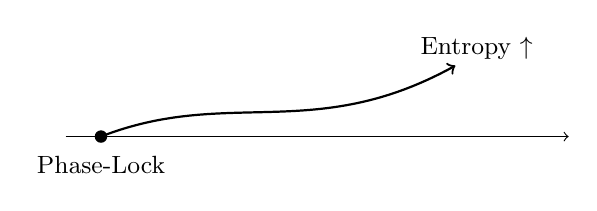
\begin{tikzpicture}[scale=0.9]
\draw[->] (-0.5,0) -- (6.6,0);
\fill (0,0) circle (2.5pt);
\node at (0,-0.4) {\small Phase-Lock};
\draw[thick,->]
  (0,0) .. controls (1.8,0.7) and (3.0,-0.1) .. (5.0,1.0);
\node at (5.3,1.25) {\small Entropy $\uparrow$};
\end{tikzpicture}

{\small Minimalist depiction of phase-lock $\to$ slippage (arrow of time).}
\end{center}

Effective “molecular chaos’’ is \textit{derived} rather than assumed:  
cycle-by-cycle coarse-graining preferentially erases backward-propagating correlators, naturally selecting the direction of increasing $\phi$-slippage.

\textbf{5. Alignment with Carroll’s “Whole Shebang.’’}  
Carroll argues that the universe may be globally time-symmetric, with arrows of time emerging only in particular regions. TCQS provides the \emph{mechanism}: local phase-lock events in the substrate generate low-entropy patches (Big-Bang-like states); the arrow is the direction of decohering away from synchronization. No cosmological fine-tuning is required.

\textbf{6. Predictions.}
\begin{itemize}\itemsep4pt
\item \textit{Direction-biased relaxation in driven time-crystal platforms} governed by tunable coherence phase fields.
\item \textit{Asymmetric correlator decay} in periodically driven cold atoms after coarse-graining $>$ one cycle.
\item \textit{Entropy–geometry correspondence:} entropy production correlates with curvature of a Fisher-like coherence metric.
\item \textit{Cosmology:} statistics of low-entropy patches follow from phase-lock likelihood, not anthropic selection.
\end{itemize}

\section*{6. Implication}
The Big Bang corresponds to a \emph{local coherence-maximal, phase-aligned region} rather than a true beginning.  
The arrow of time emerges naturally as the monotonic increase of entropy along the direction of growing phase incoherence.

\vspace{6pt}

\begin{center}
\textit{The universe does not begin with a boundary; \\
it begins, locally, with a synchronization.}
\end{center}

\vfill

{\footnotesize
TCQS Standalone Series — concise theoretical communications on coherence, cosmology, and substrate dynamics.}


\begin{center}
{\Large \textbf{Local Arrows of Time from Phase-Lock in the \\ Time-Crystalline Quantum Substrate (TCQS)}}\\[6pt]
{\small \emph{A TCQS one-page technical communication}}
\end{center}

\vspace{6pt}

\noindent
\textbf{Abstract.}  
Standard physics claims that entropy increase follows from time-symmetric microdynamics. 
However, as clarified by Boltzmann's reversibility paradox and the work of David Albert and the philosophy-of-physics community, this is incorrect: the arrow of time is not derived but \emph{assumed} through hidden low-entropy boundary conditions. This document shows how the Time-Crystalline Quantum Substrate (TCQS) resolves this foundational problem by replacing ``special initial conditions'' with \emph{local phase-synchronization events} in a globally time-symmetric substrate.

\vspace{4pt}

\section*{1. The Problem}
Microscopic laws (Newtonian, Hamiltonian, quantum) are time-reversal symmetric.  
Yet macroscopic reality displays a clear arrow: $dS/dt > 0$.  
Boltzmann's attempt to derive this via the $H$-theorem depends on the Stoßzahlansatz (molecular chaos), which—after a single collision—fails.  
Reapplying it means re-inserting the arrow by hand.  
Thus: no true derivation of the arrow exists in standard physics.

\vspace{4pt}

\section*{2. TCQS Framework}
The TCQS posits a discrete, periodic substrate with update period $T$:
\[
|\Psi(t+T)\rangle = U_F |\Psi(t)\rangle ,
\]
where $U_F$ is unitary and globally time-symmetric.  
Coarse-graining defines a coherence density $C(x,t)$ and phase field $\phi(x,t)$, whose dynamics include memory:
\[
\partial_t C = \mathcal{F}(C,\nabla C) - \Gamma[C] 
    + \int_0^t K(t-t')\,\mathcal{G}[C(t')]\,dt'.
\]
The \emph{memory kernel} $K$ originates from the time-crystal cycles and produces directional asymmetry only after coarse-graining.

\vspace{4pt}

\section*{3. Phase-Lock as ``Low Entropy''}
In TCQS, ``special initial conditions'' become \emph{local phase-lock events}.  
A domain $\Omega$ at cycle time $t_*$ satisfies:
\[
\phi(x,t_*) \approx \phi_0 \quad \forall x \in \Omega.
\]
Uniform coherence phase drastically reduces the number of compatible macrostates:
\[
S[C(t_*)] \ \text{minimal}.
\]
Thus: low entropy is not tied to a cosmological beginning, but to a \emph{phase-aligned patch} within a globally time-symmetric substrate.

\vspace{4pt}

\section*{4. The Arrow from Phase Slippage}
After a phase-lock event, the coherence phase gradients grow:
\[
\nabla \phi \neq 0 ,
\]
and the entropy functional on the coherence manifold increases:
\[
\frac{dS}{dt} \;=\; \int d^3x \; 
\sigma(x,t), \qquad 
\sigma \propto (\nabla \phi)^2 
    + \text{curvature terms from the coherence metric}.
\]
This yields an emergent, \emph{local} arrow of time:
the direction of increasing phase slippage relative to the substrate cycles.

\vspace{4pt}

\section*{5. Comparison to Standard Approaches}
\begin{itemize}
    \item \textbf{Boltzmann:} Assumes chaos; TCQS derives effective chaos from phase-biased correlation pruning.
    \item \textbf{Hartle--Hawking:} Uses an effective initial boundary; TCQS replaces this with local phase-lock.
    \item \textbf{Carroll's whole-shebang:} Global time symmetry with local arrows. TCQS provides the \emph{mechanism}.
\end{itemize}

\vspace{4pt}

\section*{6. Implication}
The Big Bang corresponds to a \emph{local coherence-maximal, phase-aligned region} rather than a true beginning.  
The arrow of time emerges naturally as the monotonic increase of entropy along the direction of growing phase incoherence.

\vspace{6pt}

\begin{center}
\textit{The universe does not begin with a boundary; \\
it begins, locally, with a synchronization.}
\end{center}

\end{document}

